
\documentclass[runningheads]{llncs}
\usepackage[text={150mm,220mm},centering]{geometry}
\usepackage{graphicx}
\usepackage{tikz}
\usepackage{float}
\begin{document}
\title{\large{CSCI814 IT Project Management (Lab5)}}
%--------------------Please do NOT change the content above.-------------------------------------------------

%
%----Please write your personal information as below.------------------------------------
%
\author{\large{Student Name: Wangzhihui Mei \\ % Please write your name here
CCNU Student Number: 2019124044 \\ % Please write your CCNU student number here
UOW Student Number: 6603385}}  % Please write your UOW student number here


%-----------------------------------------------------------------------------------------------



%---------Do not change the content of this part--------------------

\authorrunning{CCNU Wollongong Joint Institute}
\institute{Central China Normal University Wollongong Joint Institute}

\maketitle
\clearpage

%-----------Please write your solutions to the questions in the assignment from here.---------------

\section*{In-class}
\subsection*{3}
\textbf{a}

In MS Project, a predecessor is defined as a task which drives its successor task before it can start or finish. When scheduling projects, an individual task may have multiple predecessors linked to it.

\noindent\textbf{b}
\begin{itemize}
    \item Finish to Start: Predecessor must finish before Successor can start.
    \item Start to Start: Predecessor must start before Successor can start.
    \item Finish to Finish: Predecessor must finish before Successor can finish.
    \item Start to Finish: Predecessor must start before Successor can finish.
\end{itemize}

\noindent\textbf{c}
When the first activity finishes, a second activity starts. This is a Finish to Start sequence, and it is widely used in a network diagram. There are many instances when the second activity starts when the first activity is about to finish, or a second activity will start a few days after the end of the first activity. These two conditions are known as Lead and Lag.  

\noindent\textbf{d}

\noindent Flexible constraints: Project can change the start and finish dates of a task. For example, the task Select locations to film can start as soon as possible. This type of flexible constraint is called As Soon As Possible, or ASAP for short, and is the default constraint type in Project. No constraint date is associated with flexible constraints.

\noindent Inflexible constraints A task must begin or end on a certain date. For example, a task, such as Set up lighting, must end on June 14, 2008. Inflexible constraints are sometimes called hard constraints.

\noindent Semi-flexible constraints A task has a start or finish date boundary. However, within that boundary, Project has the scheduling flexibility to change the start and finish dates of a task. For example, a task such as Install props must finish no later than June 13, 2008. However, the task could finish before this date. Semi-flexible constraints are sometimes called soft or moderate constraints.

\noindent\textbf{e}
a task in one of your projects where the work needs to start, then stop somewhere in the middle of the task, and then resume at a later date

\subsection*{4}
\begin{figure}[h]
    \centering
    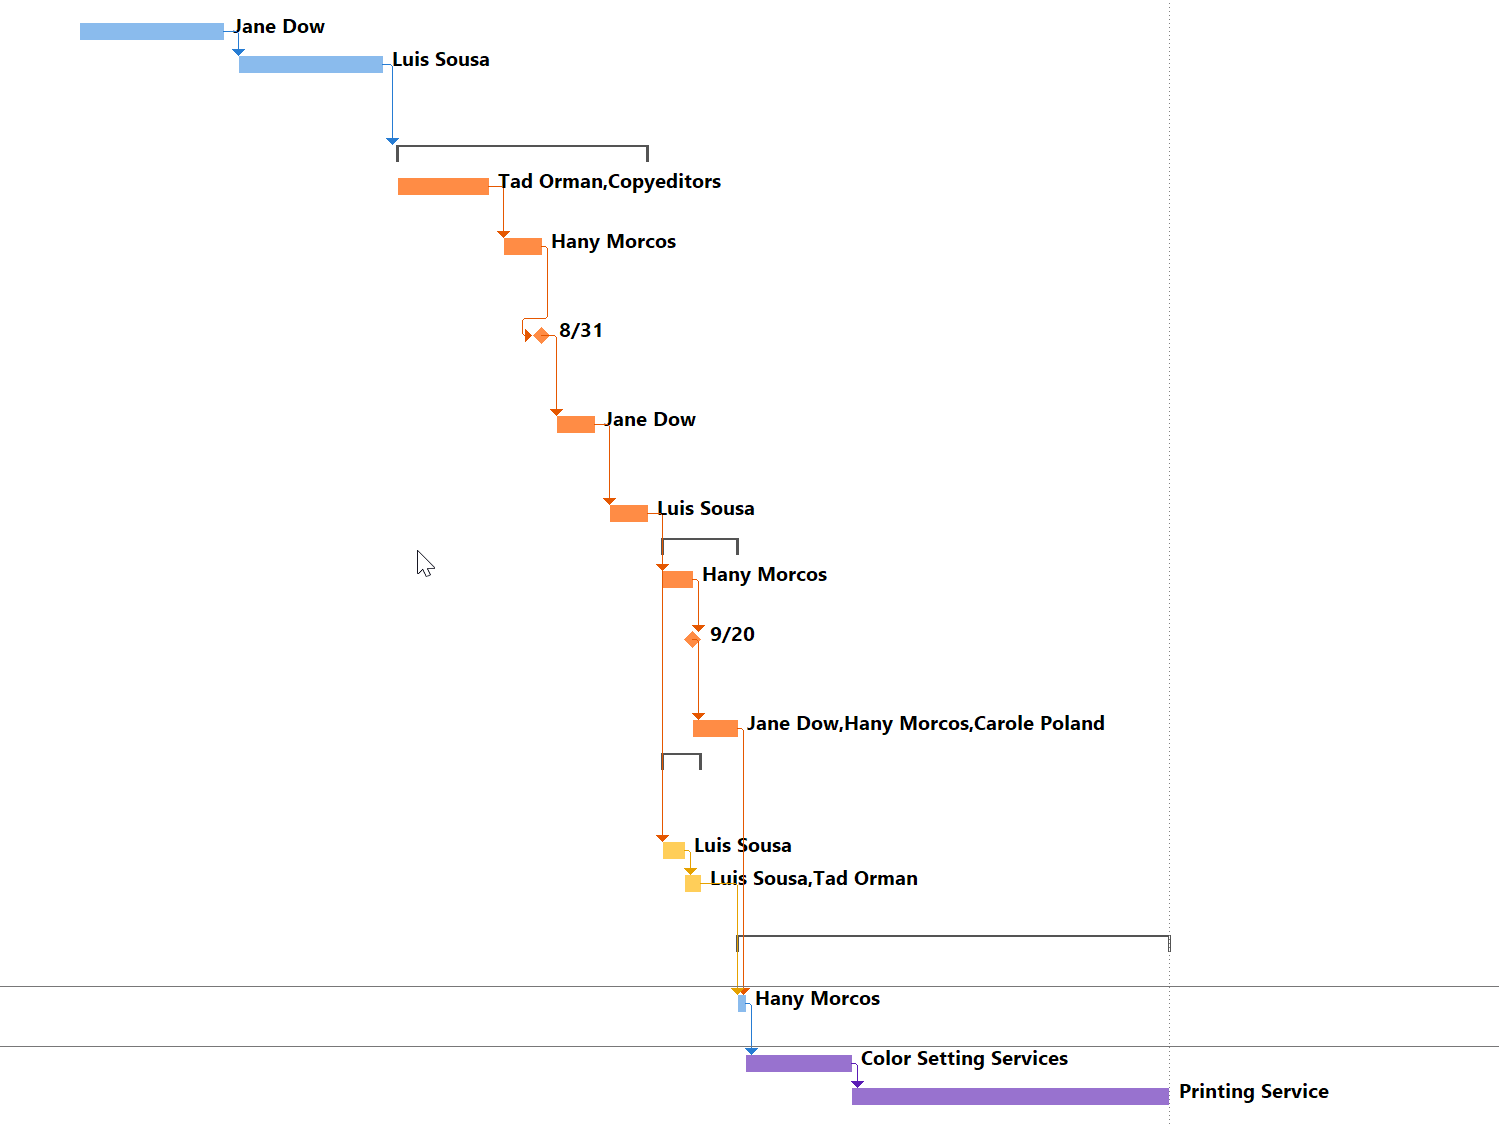
\includegraphics[width=1.0\textwidth]{image/f0}
    \caption{a}
\end{figure}

\section*{Lab5}

\subsection*{5}
\begin{figure}[h]
    \centering
    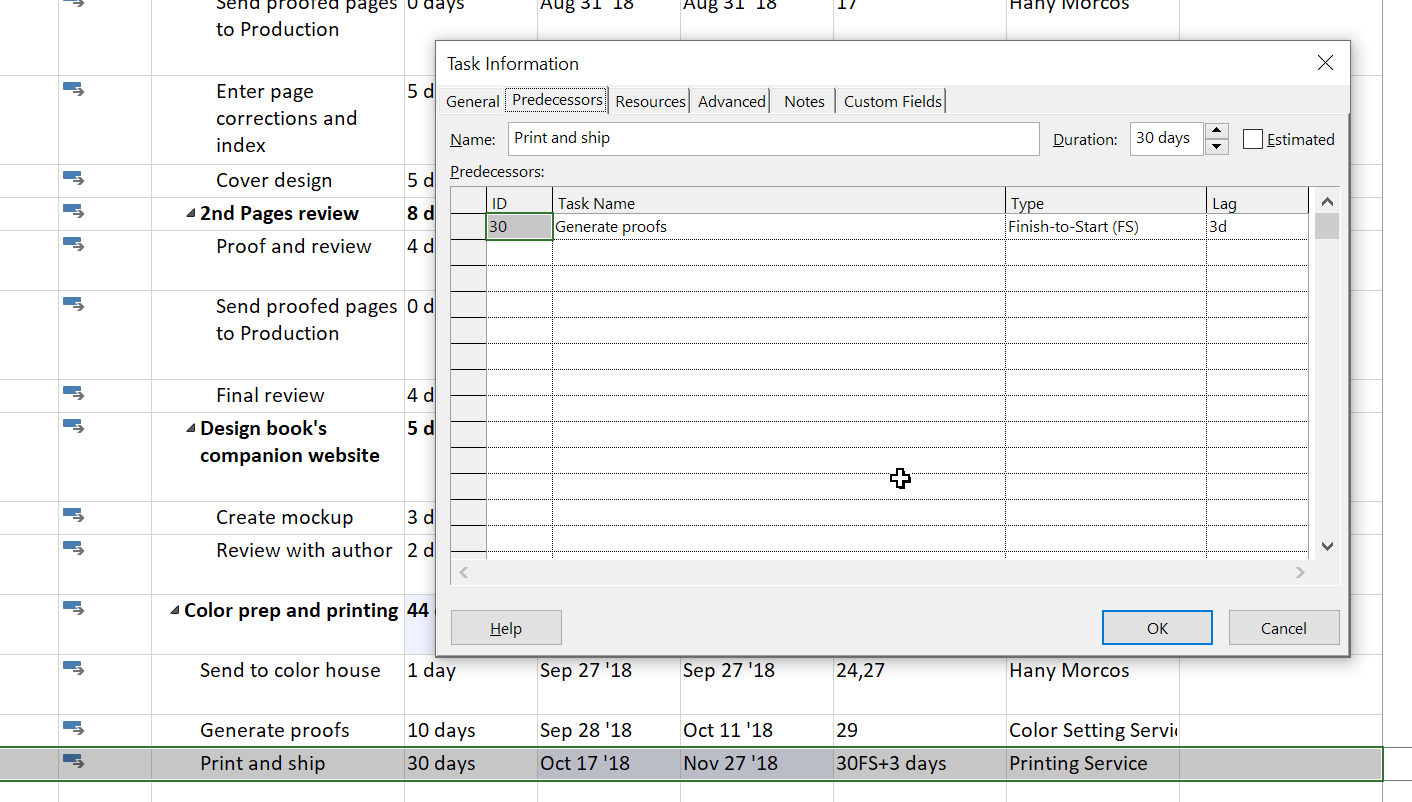
\includegraphics[width=1.0\textwidth]{image/fa}
    \caption{a. Add lag time}
\end{figure}

\begin{figure}[H]
    \centering
    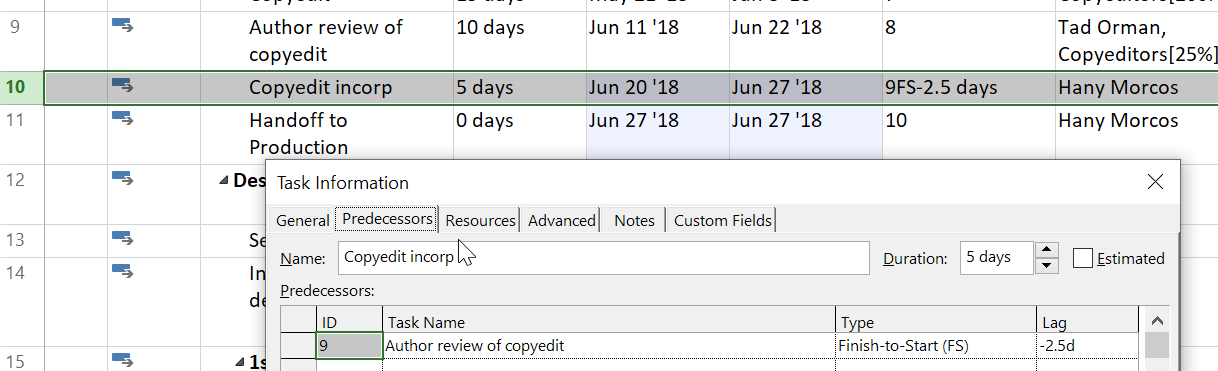
\includegraphics[width=1.0\textwidth]{image/fb}
    \caption{b. Overlap task}
\end{figure}

\begin{figure}[H]
    \centering
    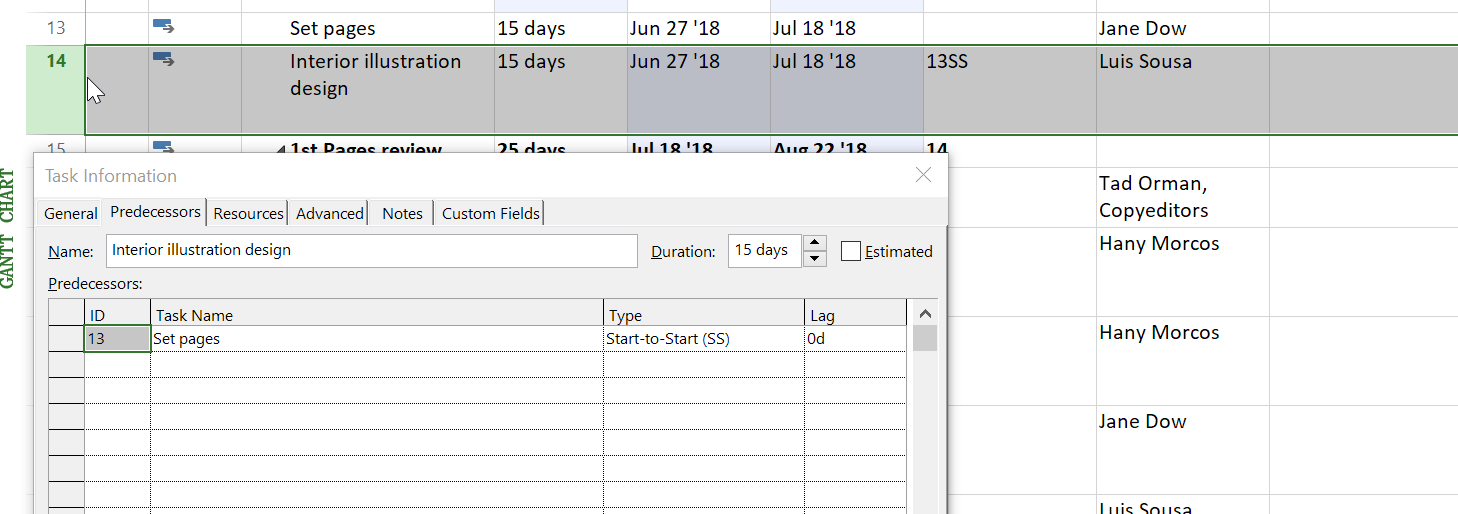
\includegraphics[width=1.0\textwidth]{image/fc}
    \caption{c. Change task relationship}
\end{figure}

\begin{figure}[H]
    \centering
    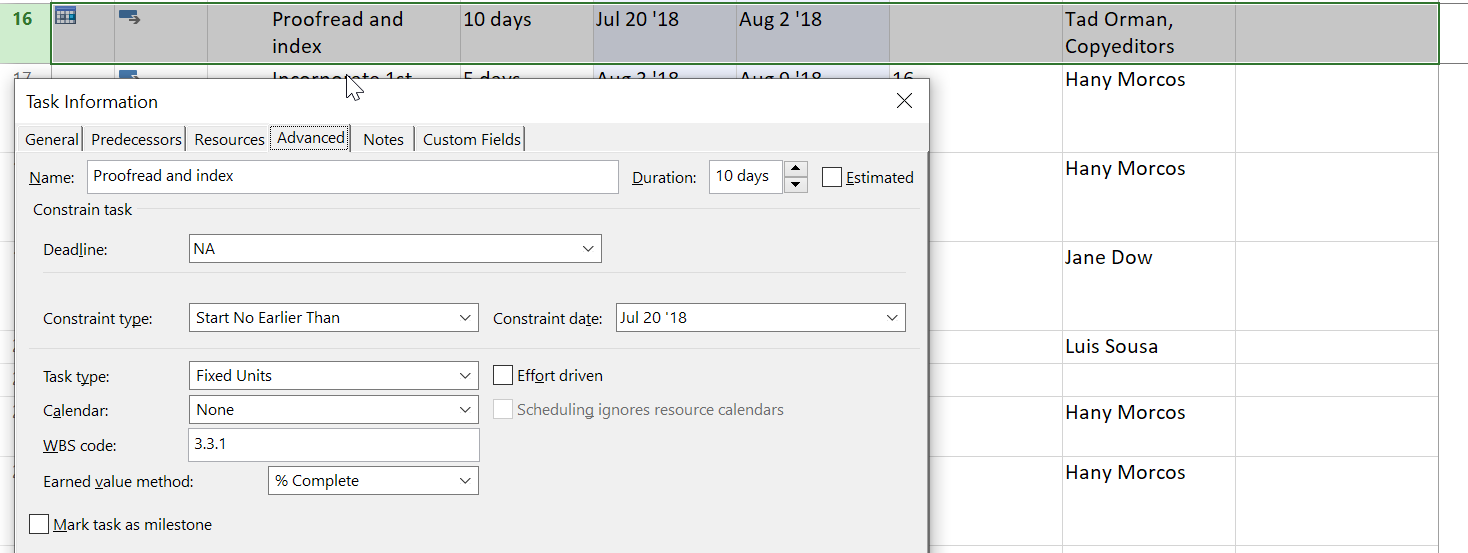
\includegraphics[width=1.0\textwidth]{image/fd}
    \caption{d. Add Constraint}
\end{figure}

\begin{figure}[H]
    \centering
    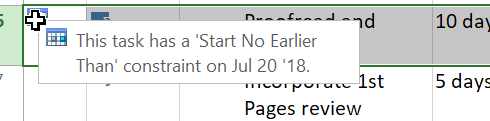
\includegraphics[width=1.0\textwidth]{image/fe}
    \caption{e. See the constraint details}
\end{figure}

\begin{figure}[H]
    \centering
    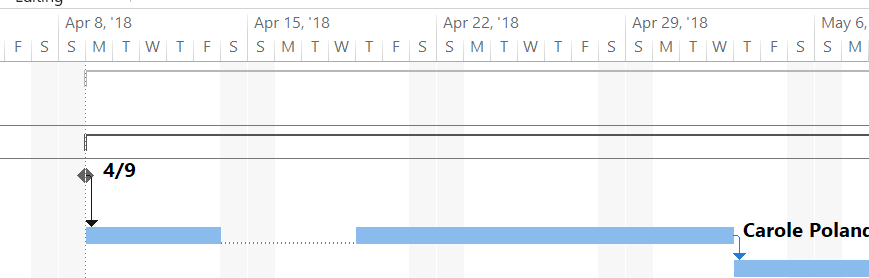
\includegraphics[width=1.0\textwidth]{image/ff}
    \caption{f. Split task}
\end{figure}

\begin{figure}[H]
    \centering
    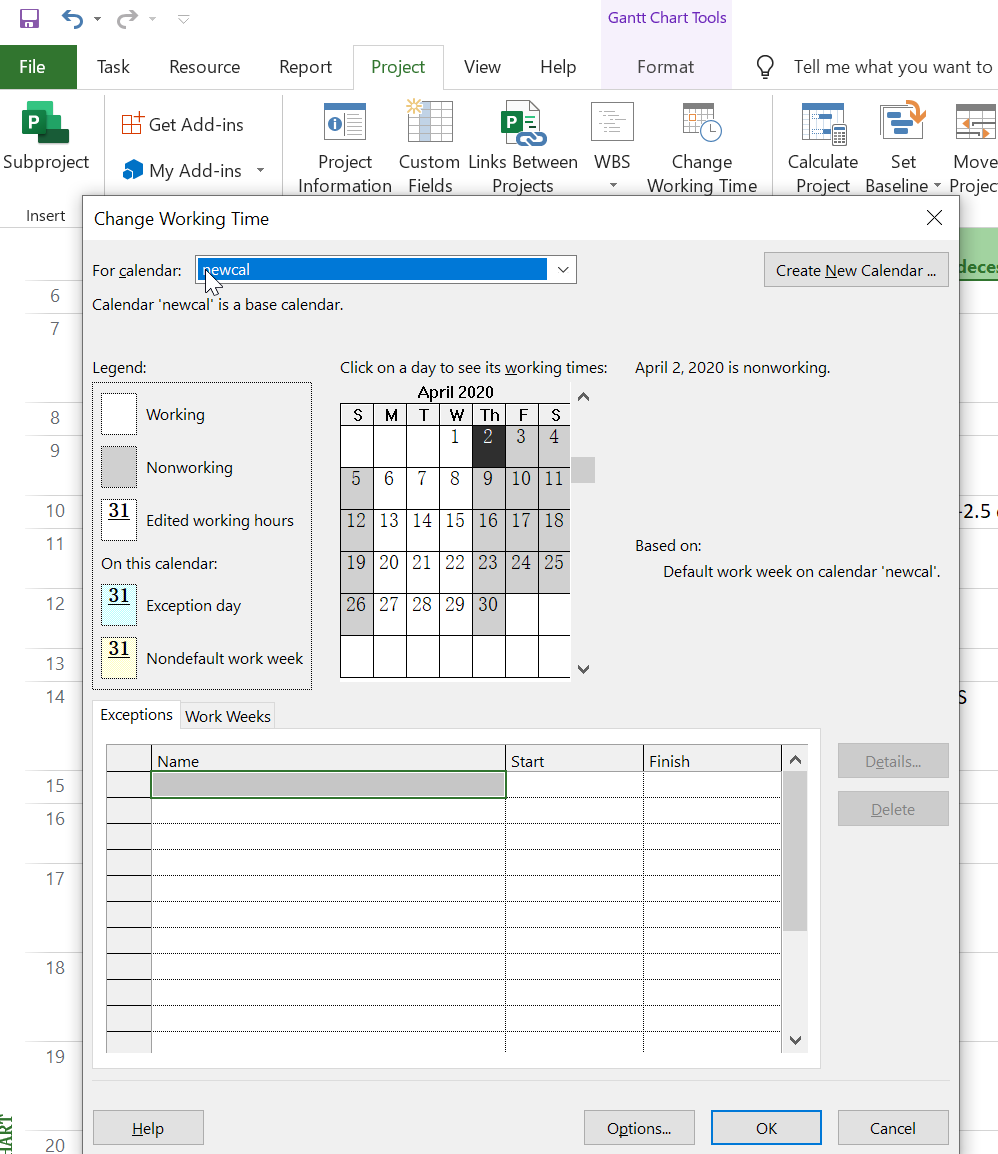
\includegraphics[width=0.5\textwidth]{image/fg}
    \caption{g. Customize calendar}
\end{figure}

\begin{figure}[H]
    \centering
    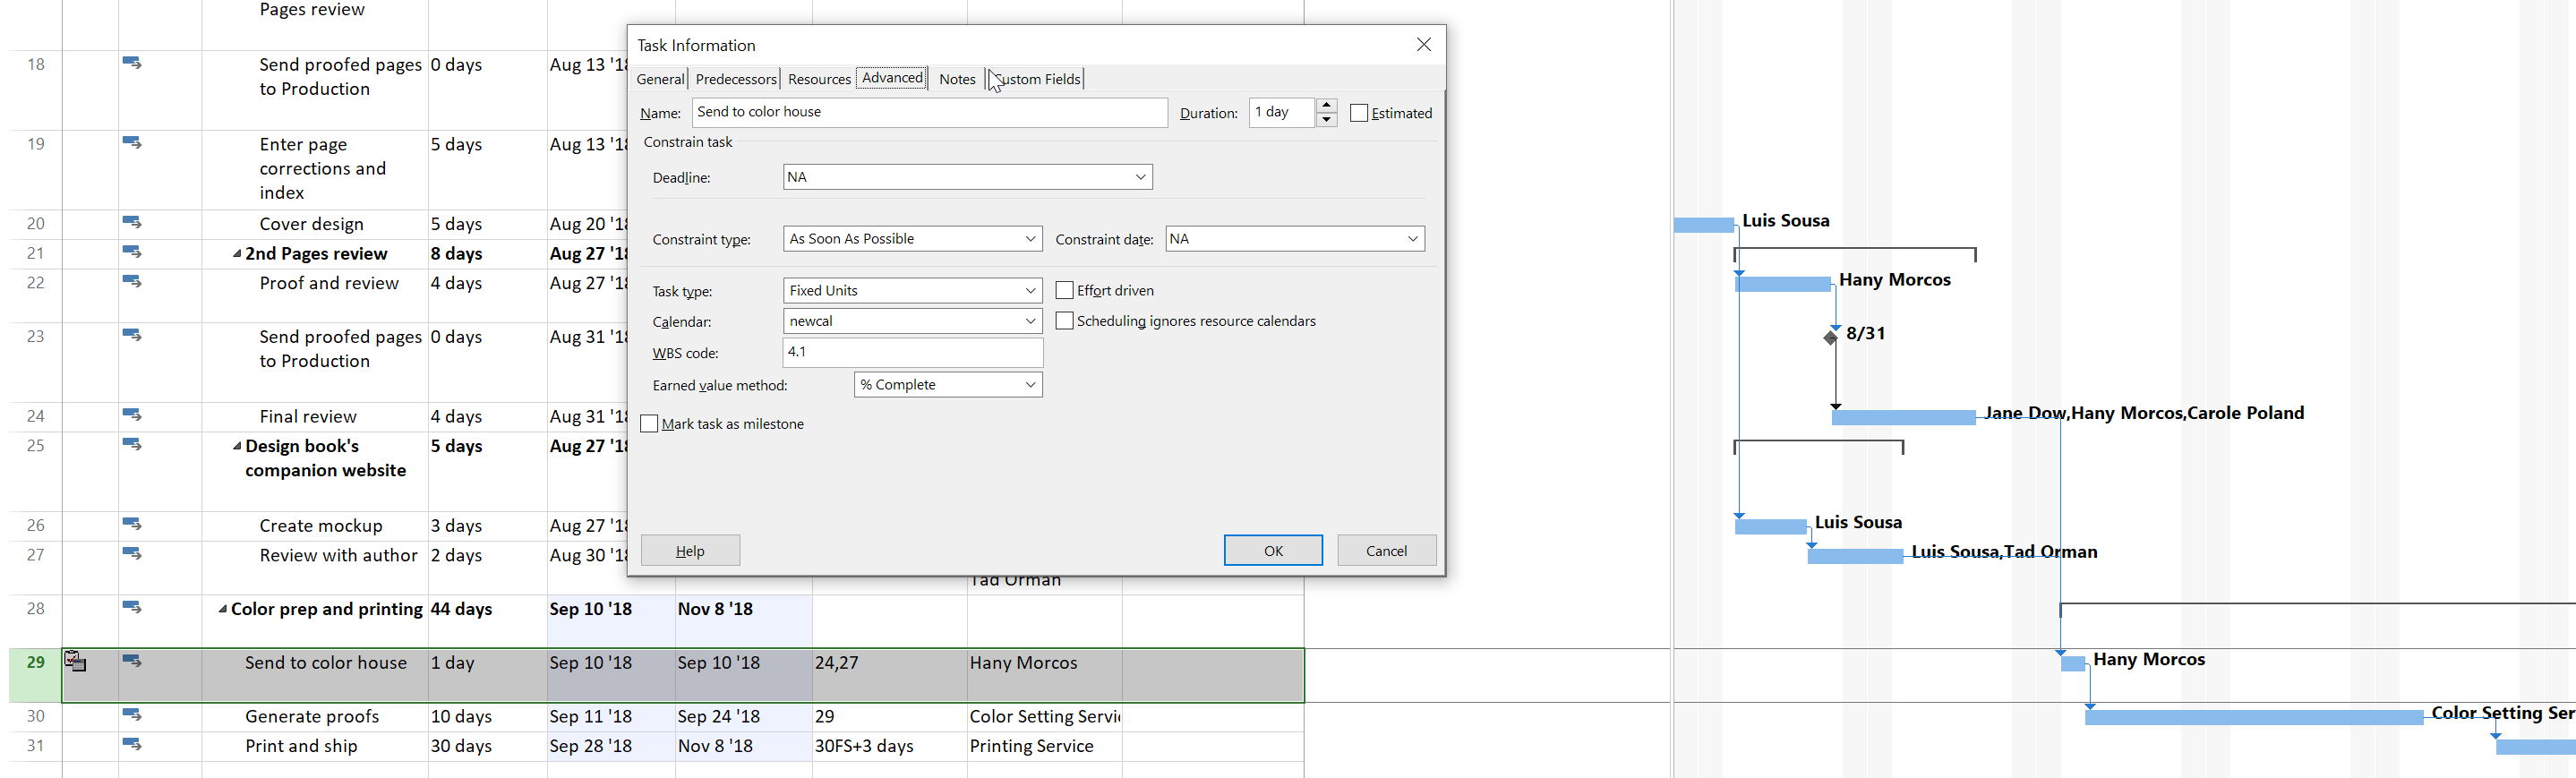
\includegraphics[width=1.0\textwidth]{image/fh}
    \caption{h. Apply calendar to task}
\end{figure}

\begin{figure}[H]
    \centering
    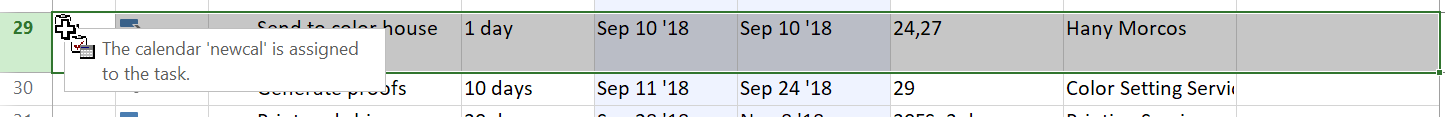
\includegraphics[width=1.0\textwidth]{image/fi}
    \caption{i. calendar icon}
\end{figure}


\subsection*{6}
\begin{figure}[H]
    \centering
    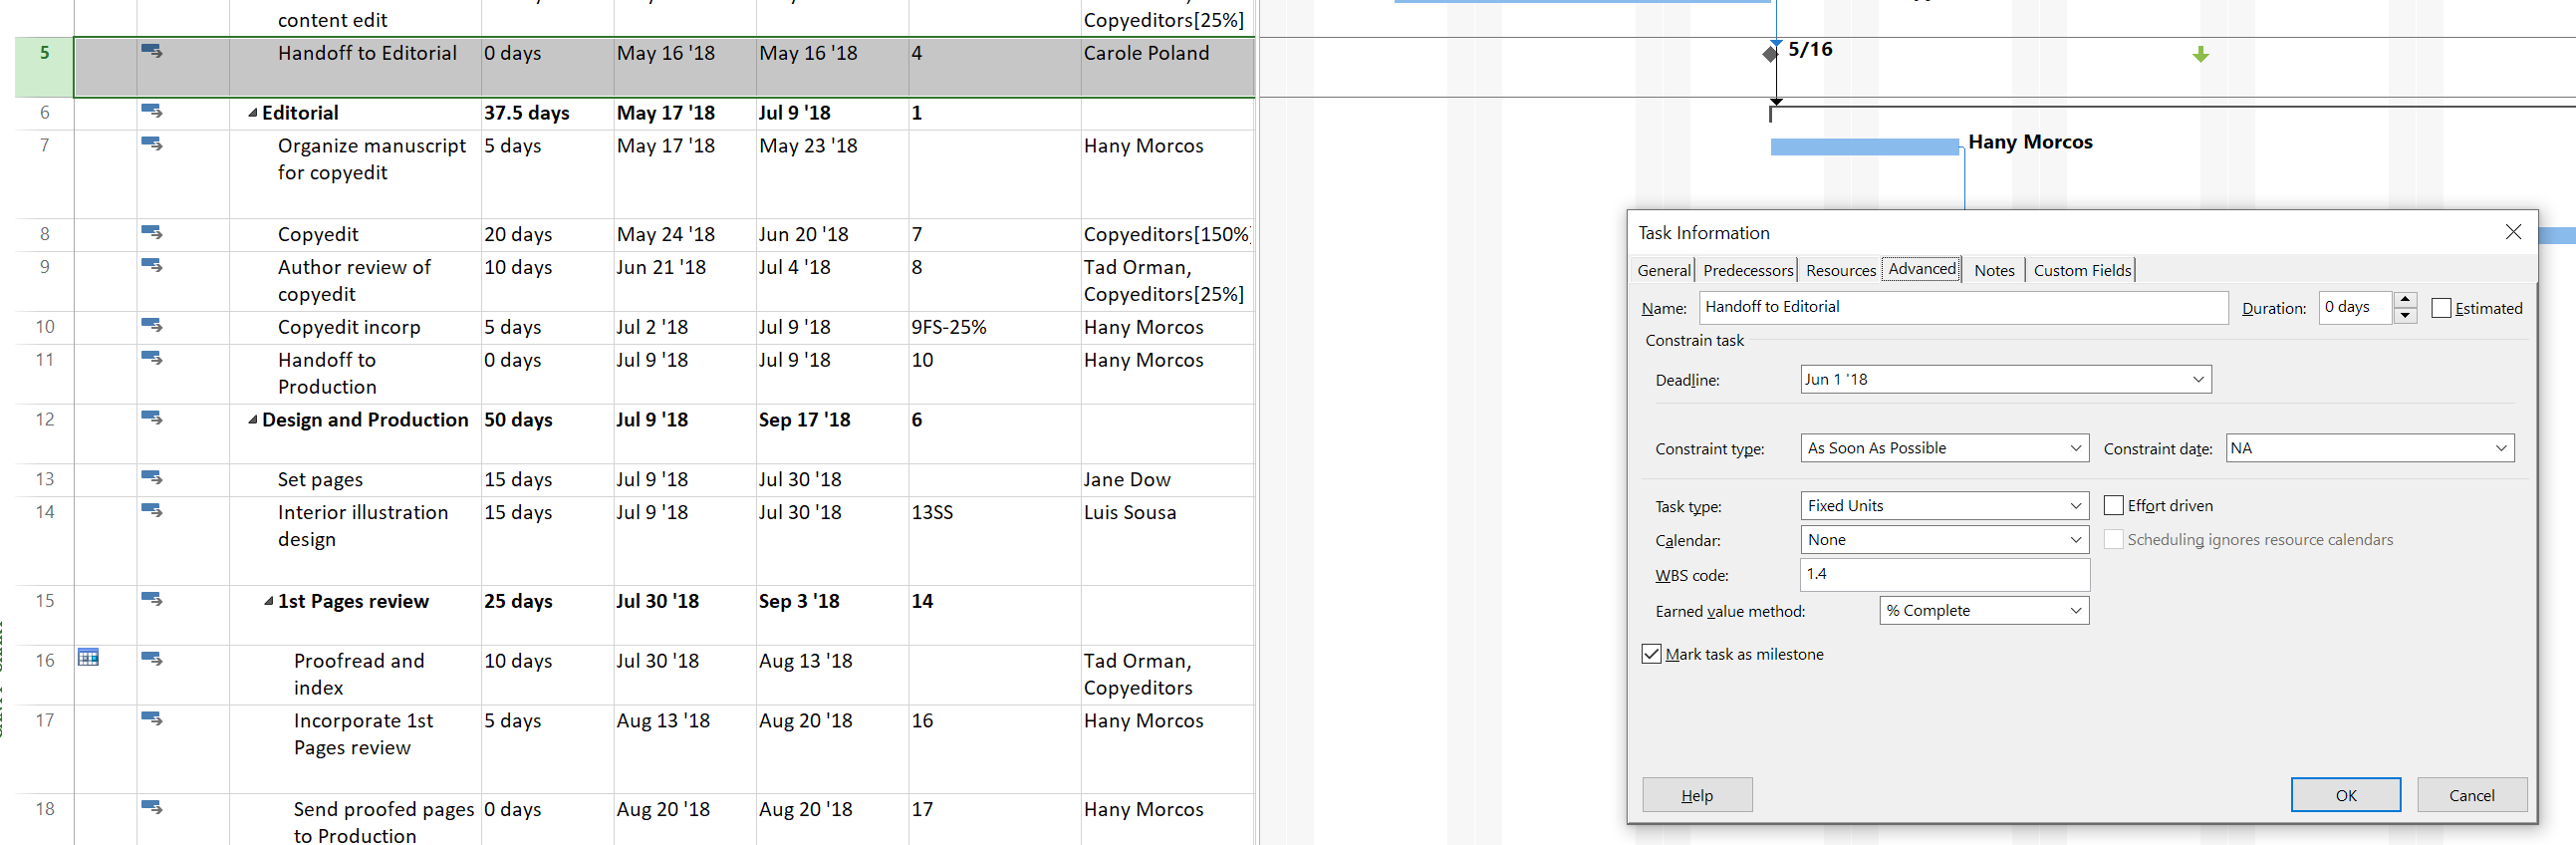
\includegraphics[width=1.0\textwidth]{image/f2a}
    \caption{a. deadline}
\end{figure}

\begin{figure}[H]
    \centering
    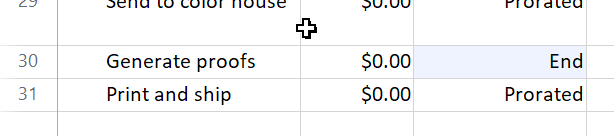
\includegraphics[width=1.0\textwidth]{image/f2b}
    \caption{b. Set the fixed cost to accrue}
\end{figure}

\begin{figure}[H]
    \centering
    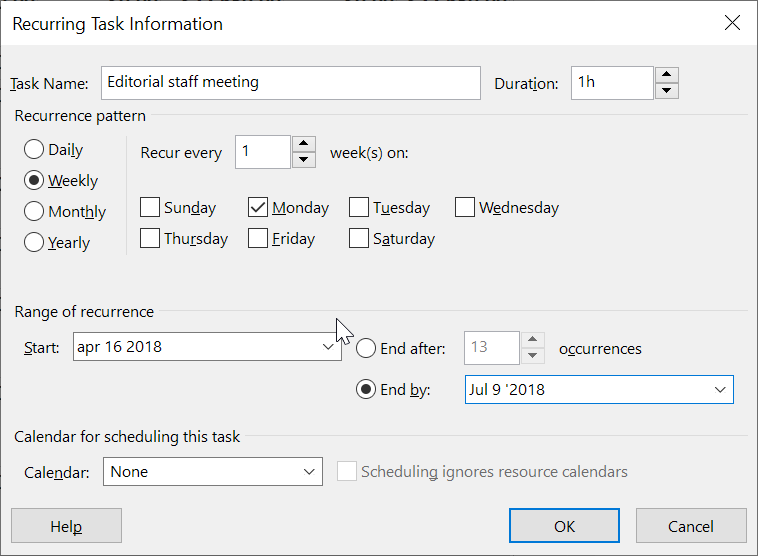
\includegraphics[width=1.0\textwidth]{image/f2c1}
    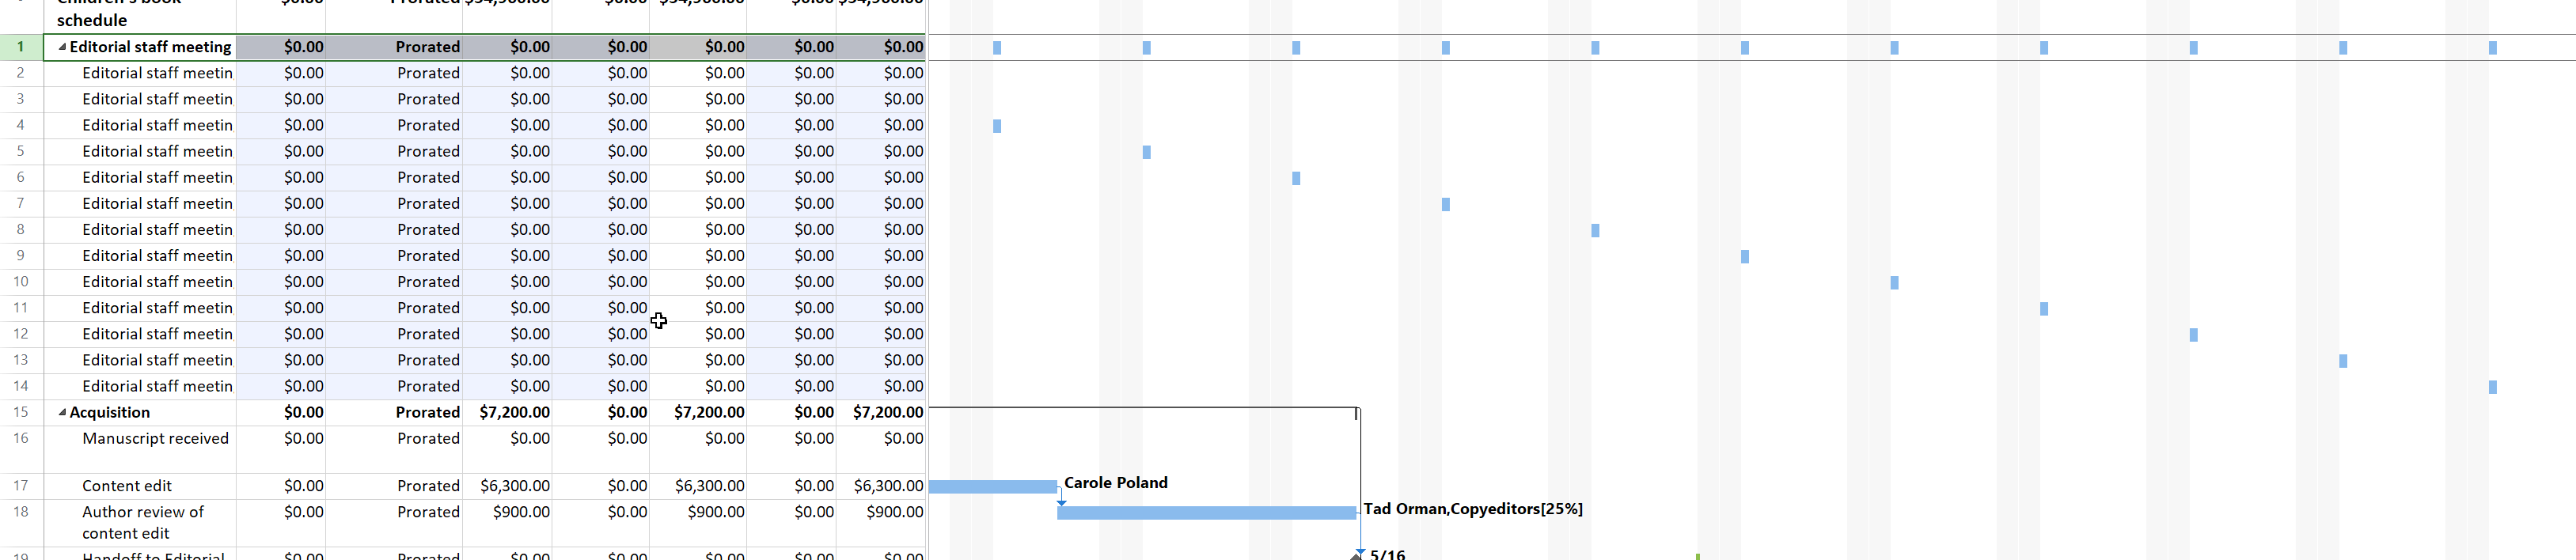
\includegraphics[width=1.0\textwidth]{image/f2c2}
    \caption{c. Add recurring task}
\end{figure}
\end{document}

\begin{figure}[H]
    \centering
    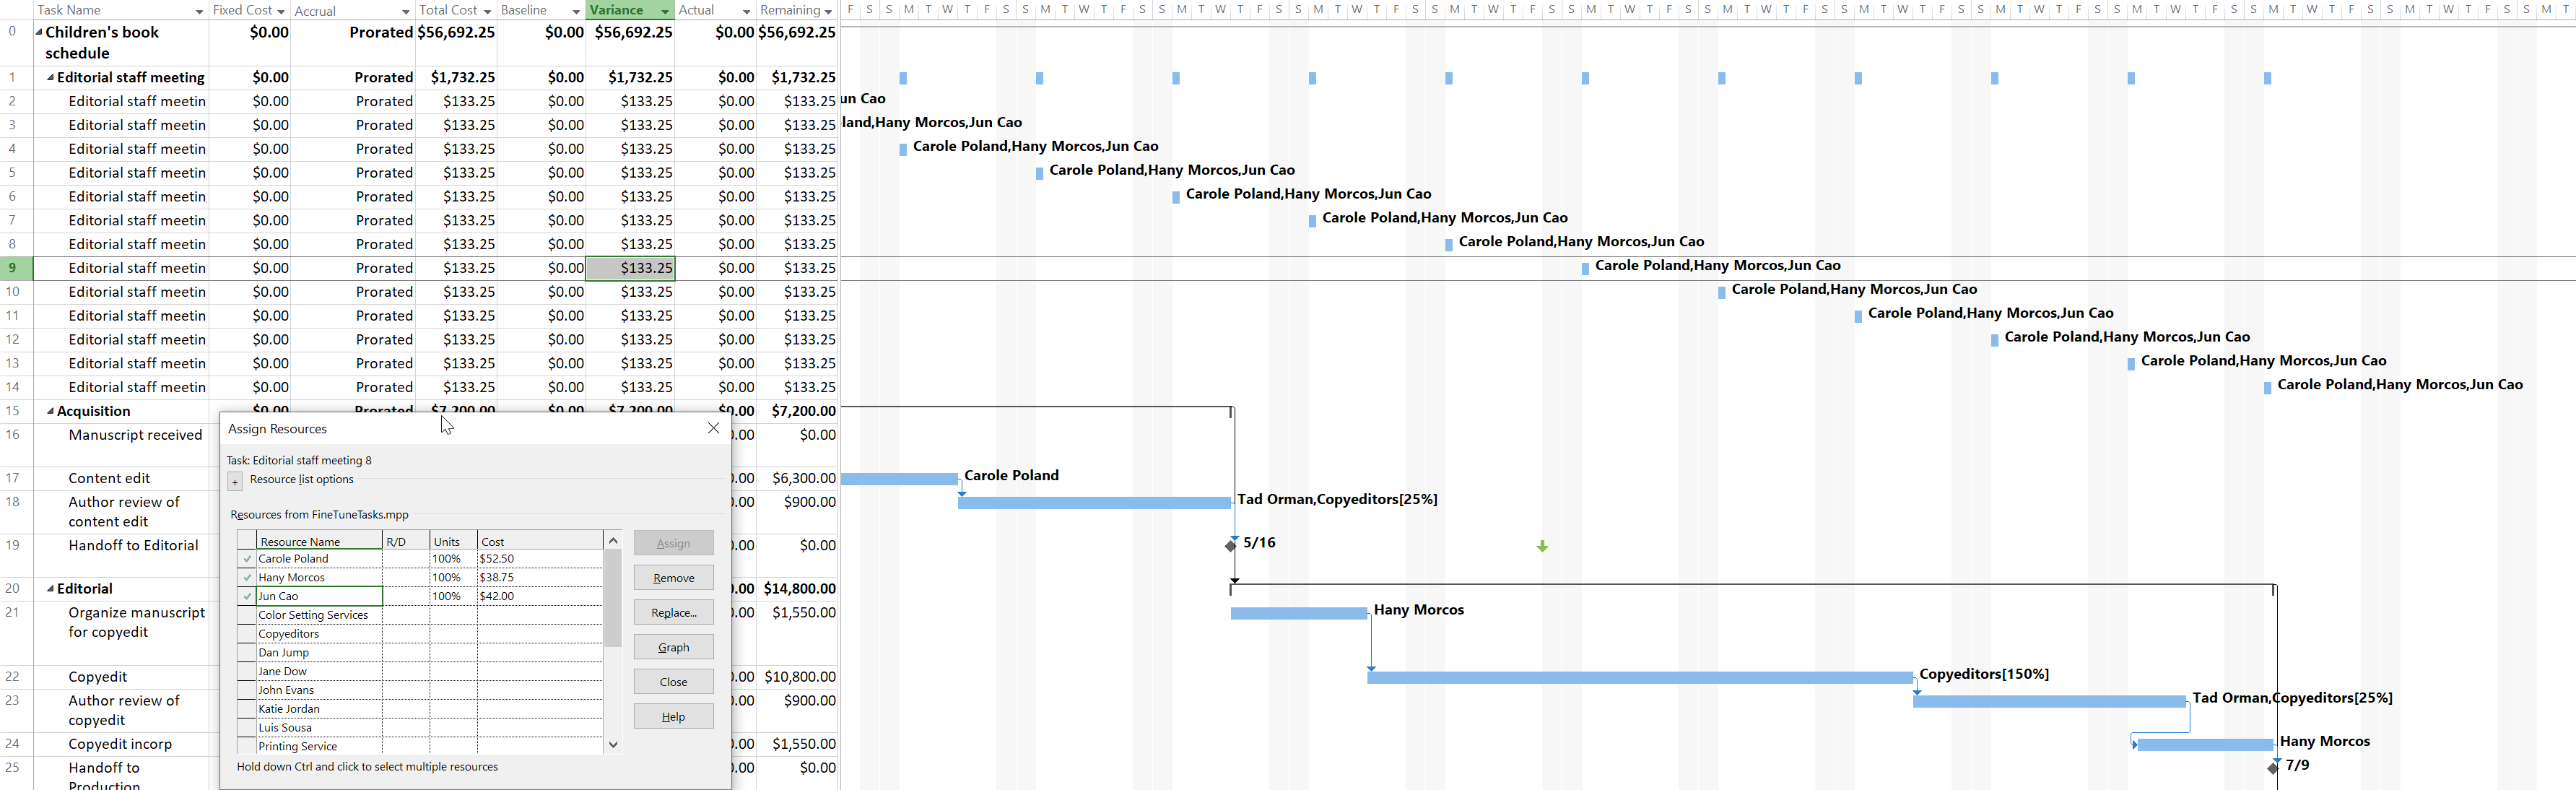
\includegraphics[width=1.0\textwidth]{image/f2d}
    \caption{d. Assign resources}
\end{figure}

\begin{figure}[H]
    \centering
    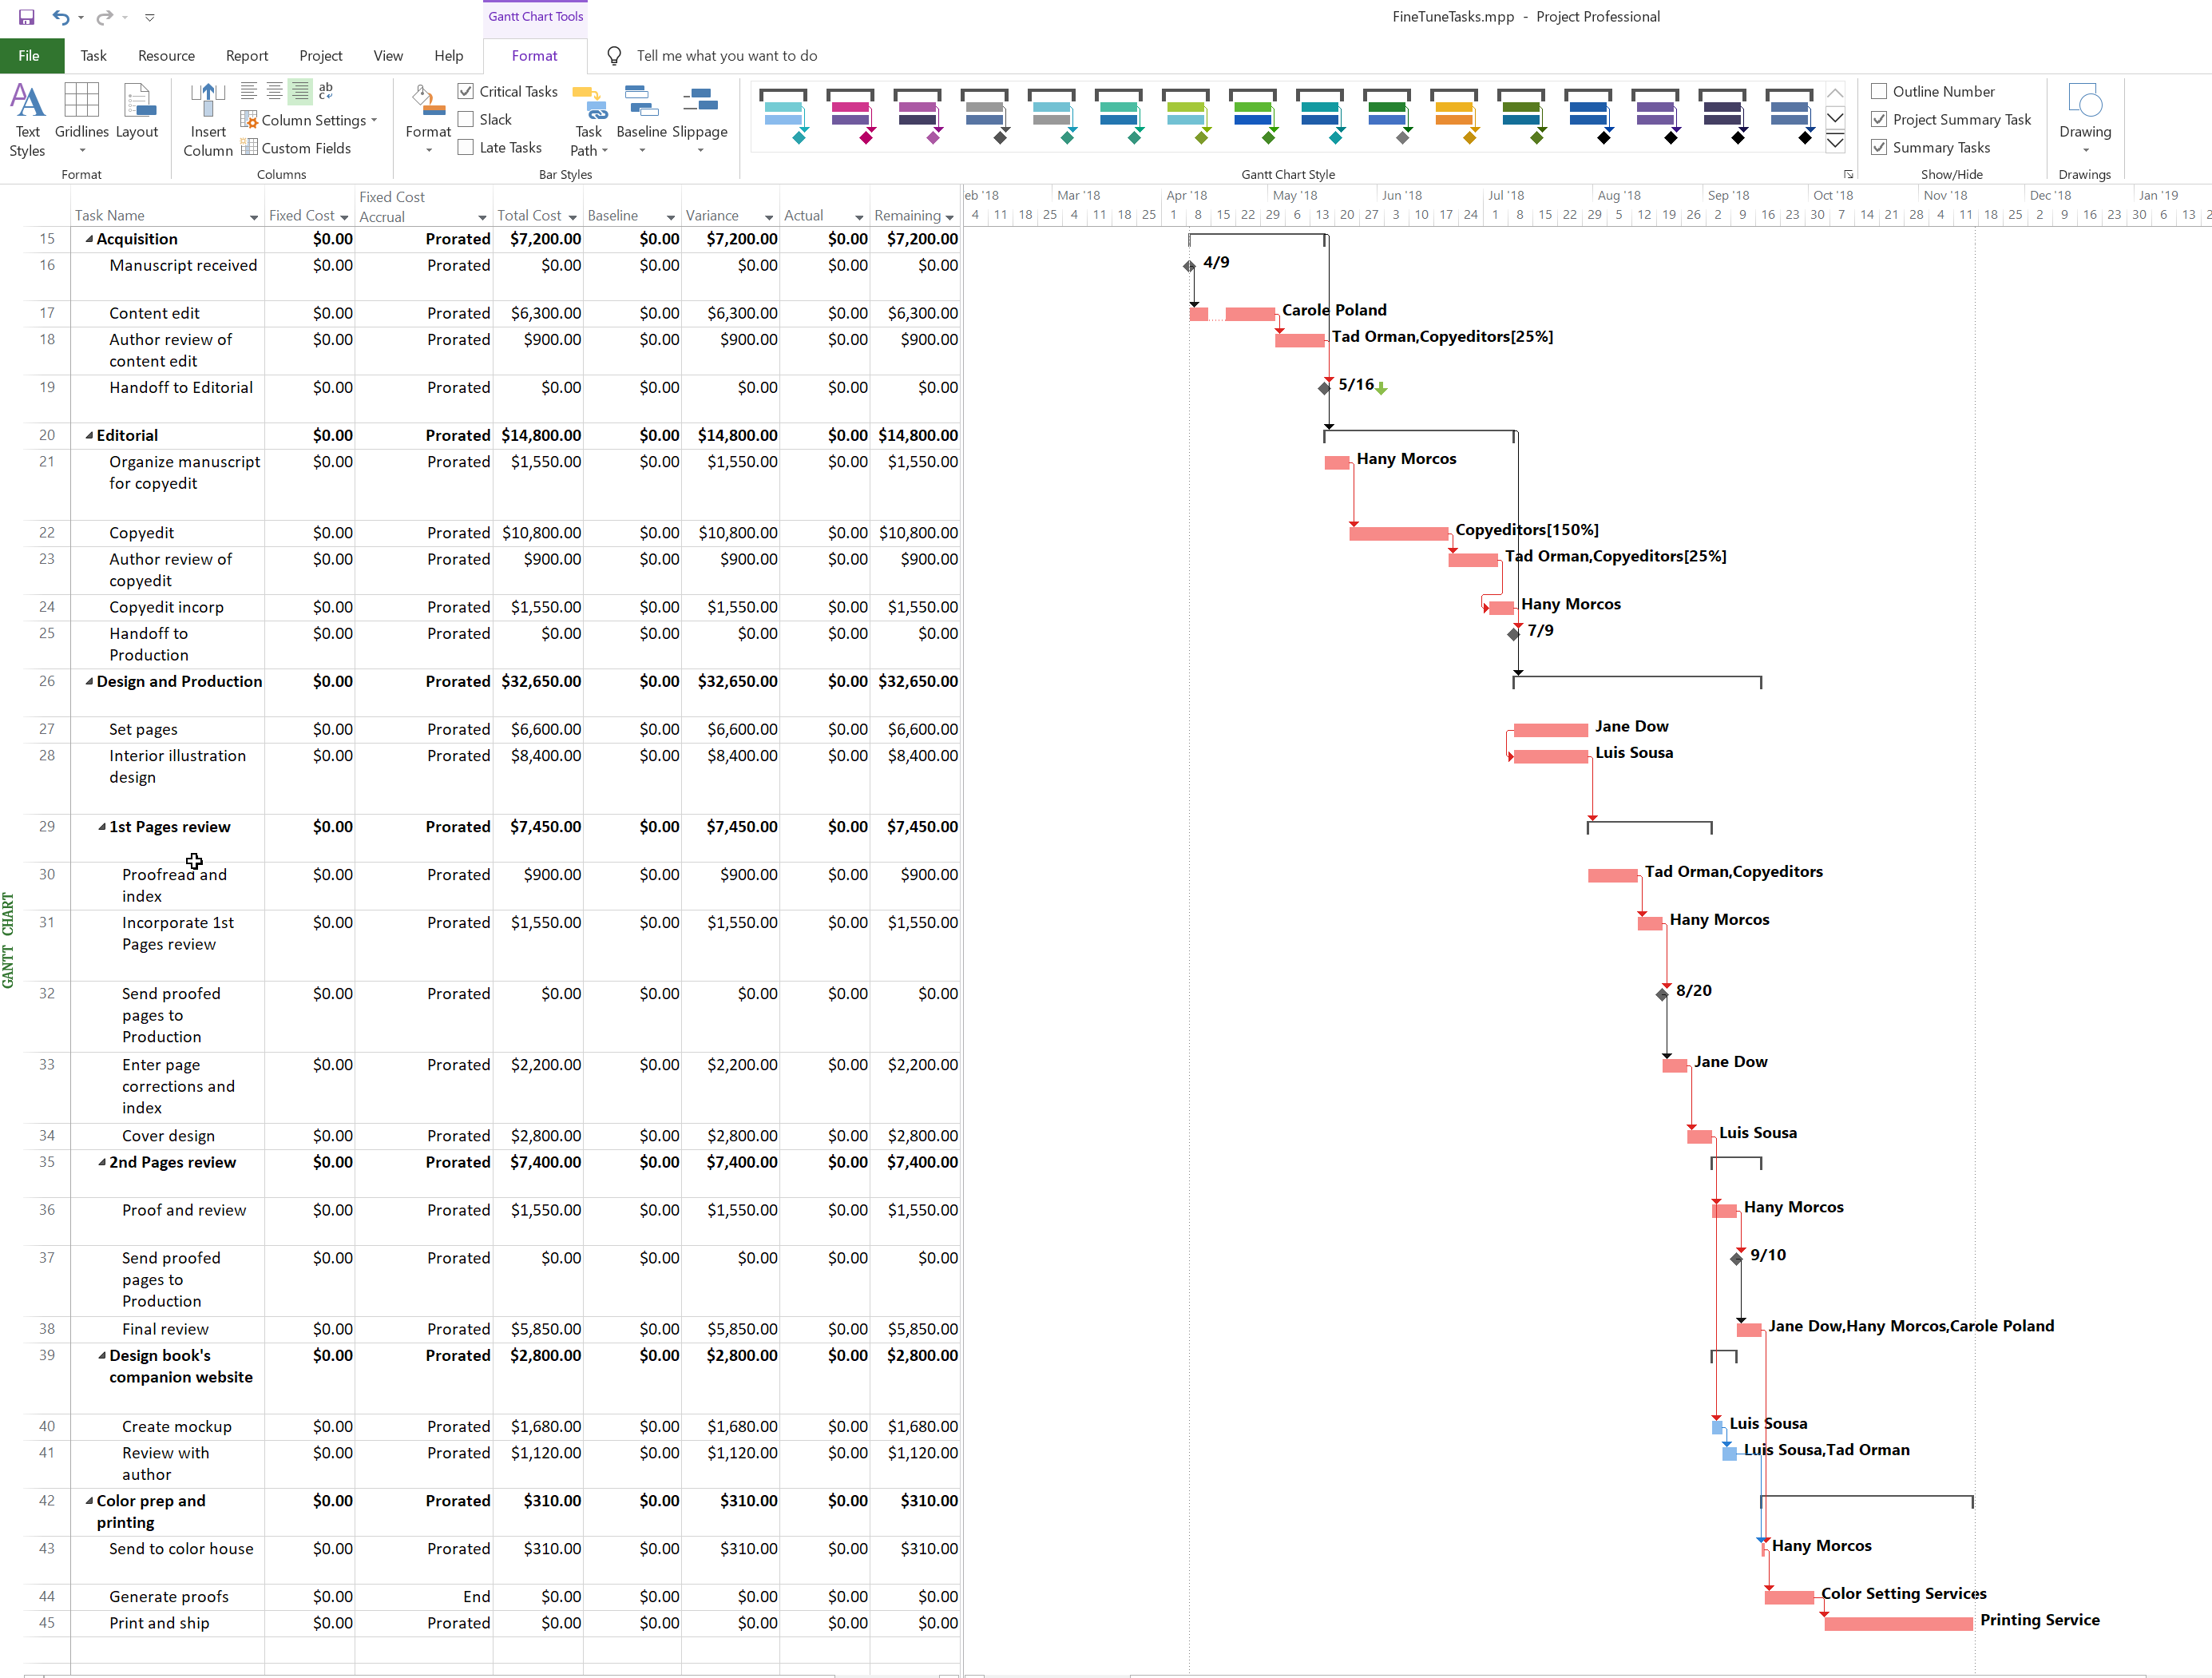
\includegraphics[width=1.0\textwidth]{image/f2e}
    \caption{e. Critical tasks}
\end{figure}
